\documentclass{article}
\usepackage{amssymb}
\usepackage{geometry}
\usepackage{graphicx}
\usepackage{placeins}
\usepackage{hyperref}
\usepackage{xcolor}

\geometry{
	a4paper,
}

\title{Ingegneria del software II}
\begin{document}
\Large
\tableofcontents
\section{Modulo I - Machine Learning for Software Engineering}
\section{Ripasso: introduzione a SVN e Github}
Un sistema di controllo delle versioni tiene traccia dei cambiamenti ad un file ed inoltre permette di tornare indietro nelle versioni. Ci sono due tipologie:
\begin{itemize}
\item Centralizzata: SVN, utenti condividono una repository che è su un solo server centralizzato
\item Distribuito: Git, ognuno ha una copia della repo.
\end{itemize}
Differenze con classici sistemi di storage cloud sono varie:
\begin{itemize}
\item SVN e Git sincronizzano solo se c'è richiesta, mentre per sistemi cloud avviene in automatico
\item I merge sono a grana fine per SVN e Git, per Dropbox/Drive è a grana più spessa.
\item La storia delle versioni è mantenuta da SVN e Git, mentre poterebbe non esserlo per Dropbox/Drive
\end{itemize}
Working copy: versione su cui è possibile lavorare in locale. Non si lavora mai sulla risorsa condivisa, bensì su quella locale. \\ Revisione: particolare stato della risorsa condivisa, su cui è possibile tornare indietro. La versione è spesso una revisione particolare, che può essere offerta agli utenti (es versione 1.0 può corrispondere alla revisione 150).
\subsection{Issue tracking systems}
Sistema che permette di creare, assegnare e tenere traccia dei problemi (issues). Tutto nasce da Bugzilla (per progetti open source), un bug in un codice è molto simile a descrivere un requisito: nasce il concetto di ticket. Un ticket è un informazione rilevante al progetto, come un requisito da implementare o un bug.\\ Molti sistemi sono gestiti attraverso i ticket (medie-piccole dimensioni), ogni ticket ha un workflow: creato, assegnato, sviluppato, testato, approvato, chiuso. Tra gli esempi di sistemi per issue tracking ci sono Jira, Github, Redmine.
\section{Tecniche di Machine Learning ed analisi software a supporto della quality assurance e del testing}
I bug software costano circa 2.84\$ dollari ogni anno. Il codice viene scritto in diversi linguaggi, da tantissime persone, per poter fixare bug, aggiungere nuove feature e migliorare la qualità del codice. Il software è rilasciato con grande velocità, si vuole prevenire di avere bug in modo da avere technical debt basso.\\ Failure: comportamento osservato dall'utente e che non corrisponde alle specifiche del sistema. Un difetto software è quella parte di codice che può dare luogo ad una failure, questo non avviene sempre, ma solo sotto determinate condizioni. Per evitare le failure si cerca di individuare i bug prima che questi possano essere eseguiti dagli utenti.\\ È importante capire, avendo tempo limitato, come poter priorizzare le risorse di analisi. Si parla di software analytics come analisi di dati che riguardano progetti software.\\ Un aspetto importante è ML per poter predire ed evitare i bug futuri. In generale:
\begin{itemize}
\item Misuro i dati
\item Analizzo i dati e creo il modello di ML
\item Identifico quale classe/metodo è buggy
\end{itemize}
I dati sono gestiti da i version control systems ed issue tracking systems.\\ Importanti i commenti dei commit: invece di descrivere la modifica effettuata, faccio riferimento al ticket sul sistema. Dovrebbe esserci una relazione 1-a-1 tra ticket e commit: prendo il ticket e lo sviluppo per intero, in modo poi da fare il commit delle mie modifiche.\\ Se ho il tracciamento preciso tra ticket e codice che ho implementato per quel ticket, posso vedere se l'ammontare di linee di codice richieste per realizzare il ticket è maggiore o minore di quelle richieste per rimuovere il bug. Posso differenziare i ticket in base a bug e requisito e vedere il numero di righe cambiate.\\ Una volta estratti i dati, posso collezionare molte metriche a riguardo:
\begin{itemize}
\item Quante righe di codice modificate
\item Chi le ha modificate
\end{itemize}
\subsection{Metriche per individuare bug}
Posso usare metriche per fare delle stime su quale classe è buggy:
\begin{itemize}
\item relative al codice: classe con molte righe è potenzialmente buggy
\item processi: se file è stato affetto da molti cambiamenti
\item fattori umani: se file è stato toccato da sviluppatori esperti o non.
\end{itemize}
Posso leggere tutte queste info tal ticket di JIRA, ogni commit avrà un suo identificativo.\\ Si cerca di andare a capire quali file di una release sono defective o non defective. Avrò quindi dei dati che darò in pasto a modelli di machine learning black-box, con cui potrò capire dato un nuovo file quanto questo sarà defective.
È anche importante capire perché un file è difettoso, ci sono anche regole di normativa per cui se si usa una predizione bisogna anche fornire il perché della predizione. È possibile anche vedere il perché una classe ha avuto una certa probabilità di essere difettoso.
\subsection{Process control chart}
Chart che mostra la stabilità degli eventi nel tempo: è importante che sull'asse verticale ci sia l'elemento di cui si vuole controllare la stabilità, mentre sull'asse orizzontale ci deve essere qualcosa che possa essere misurato.\\
Voglio vedere se un certo progetto ha dei difetti per in base al numero di revisione: metto su asse x il tempo (es settimane, o le revisioni), asse y avrò i difetti. Mi chiedo se in un progetto i difetti sono lineari in base alle revisioni. Dobbiamo:
\begin{itemize}
\item Selezionare i dati sull'asse y ad esempio il numero di commits o requirements 
\item Seleziono dati per asse x, asse temporale. Può essere giorni/mesi o anche release
\item Colleziono i dati
\item Calcolo media e varianza, imposto poi degli assi di limiti superiori ed inferiori (ad esempio):
\begin{itemize}
\item limite superiore (upper control limit): media + $3\cdot$deviazione standard
\item limite inferiore (lower control limit): media - $3\cdot$deviazione standard. Può andare sotto 0, alle volte conviene andarci ma altre volte no (quindi lo si fa fermare a 0).
\end{itemize}
\end{itemize}
Visualizzando il chart, posso capire se qualcosa è andata particolarmente male: quando un punto è al di fuori del limite, è significativamente diverso da tutti gli altri punti. Quindi in questo caso si analizza il perché per una determinata release c'erano dei valori così estremi, ad esempio perché c'è stato un numero così elevato di difetti.
\subsection{Ripasso: continous integration e travis}
Pratica per cui i membri del team integrano il loro lavoro continuamente. Ogni integrazione è verificata con un build del progetto, viene fatto per evitare errori nell'integrazione del progetto.\\ È molto importante che il built sia automatico, in modo che chiunque possa effettuarlo, e non solo alcuni membri del team. Importante anche che la built sia self-testing, e che inoltre i commit avvengano quotidianamente o almeno per ogni feature.\\ I test vanno effettuati in un ambiente che sia il più possibile simile all'ambiente di production: ad esempio, se ho sviluppato un app, il production environment sarà il dispositivo dei miei utenti.
\subsection{Ripasso: technical debt}
Applicazione di concetti finanziari al dominio del software engineering. Code smell e regole di qualità: una regola di qualità è un principio che detta come il codice dovrebbe essere, ad esempio:
\begin{itemize}
\item alta densità di commenti
\item bassa densità di codice
\item if statement non difficile da leggere
\end{itemize}
Una violazione o code smell è una porzione di codice non perfetto. È importantissimo soffermarsi sulla differenza fra difetto e code smell: difetto può dare vita ad un failure (sotto determinate condizioni), mentre il code smell è qualcosa non osservabile dall'utente (ad esempio la lunghezza di un if statement). Il problema è che i code smell impattano gli sviluppi futuri.\\ Il debito tecnico può essere visto come un qualcosa che darà problemi a sviluppi futuri (impatta la prossima release), può emergere organicamente come molti sistemi aumentando di complessità, aumentano la loro complessità di gestione. Inoltre, può anche essere scelto in maniera opportunistica, ovvero decidere deliberatamente di avere una certa quantità di debito tecnico.\\ Il technical debt consiste in due parti:
\begin{itemize}
\item principio: costo per eliminare i code smells
\item interesse: la penalità da pagare in futuro per il debito non eliminato
\end{itemize}
Come gestisco i code smell attraverso i ticket: tutto ciò che bisogna fare deve essere scritto in un ticket. Non c'è altro mezzo di informazione che il progetto può usare, linee guida e processi aziendali possono essere documentati su un altra piattaforma (confluence, per completare JIRA).Se c'è un code smell, \textbf{dipende dal processo aziendale}: può essercene uno che dice che chi ha introdotto lo smell lo toglie senza ticket, un altro che dice che i problemi rilevati da Sonar Cloud verranno analizzati a parte da specifiche persone che avranno il ruolo di aprire i ticket appositi. È possibile impostare i repository in modo che rigetti i commit che violano alcune regole di qualità (configurando Travis/Jenkins), così saprò che il codice è sempre smell free.
\subsection{Misure di analisi}
Voglio rispondere alla domanda: le linee di codice per le feature, sono state di più o di meno di quelle usate per risolvere i bug? Quando gestisco i dati, posso farlo per due motivi:
\begin{itemize}
\item guardare al passato: perché spendo molte LOC per risolvere i bug? Vado a fare delle analisi introspettive sul progetto
\item avvento del ML, predico il futuro: prendo delle decisioni nel presente, in modo che l'impatto dei cambiamenti futuri sia controllato
\end{itemize}
\section{Merging JIRA con Git}
\subsection{Git: comandi utili}
Una volta effettuato il clone di una repository, è possibile avere accesso al log: \textbf{git log $<$options$>$}, da accesso ai cambiamenti mostrando
\begin{itemize}
\item autore del commit
\item cambiamento
\item commento 
\end{itemize}
se non viene specificato il branch, git ritorna il log di quello corrente. Una cosa interessante può essere comparare due commit fra loro, per vedere i cambiamenti: tramite il comando \textbf{git diff $<$commit\_id$>$..$<$altro commit\_id$>$}. Alcune visualizzazioni sono human readable, ma nel codice che fa l'analisi automatica non è importante.\\
Data la revisione di un file, per ogni riga è possibile risalire al commit che ha inserito quella determinata riga: ho un file di 10 righe, mi chiedo chi ha inserito una riga, quando e perché. \textbf{git blame $<$filename$>$} (con -w ignora gli spazi bianchi). Fornisce la data dell'ultima modifica con la relativa modifica (ci sono anche meccanismi per andare indietro) e chi l'ha effettuata. È possibile fare il grep sul testo, in modo da cercare solo specifiche parti di interesse del log.
\subsection{Cercare ticket in JIRA}
Una volta trovato un progetto, è possibile selezionare il tipo di ticket da cercare, lo sviluppatore etc... (numerosi filtri), in advanced è anche possibile creare delle query SQL-like, con cui è possibile creare delle ricerche sofisticate e metterle da parte.
\section{Snoring and proportion}
Quando vedo un commit per un ticket di tipo bug, che ha toccato 3 classi, so che quelle 3 classi prima del commit erano buggate prima del commit. Con il blame so qual è il commit preciso che ha prodotto un determinato stato di una riga. In generale, la predizione dei difetti cerca di individuare quale artefatto software è più propenso a mostrare difetti: ci mettiamo nei panni di chi deve testare la release finale (molte classi) per capire quale classe è opportuno testare. Vorremmo una stima di quanto una classe è probabilmente buggy, per ordinarle in modo crescente (per probabilità).\\ Prima di poter fare delle stime, è necessario misurare cosa stimare: quando si fa una predizione: un conto è farla binaria, un altro è se vanno predetti dei numeri. Quest'ultima è estremamente più complessa di quella binaria.\\ esempio: supponiamo di dover predirre il meteo, a seconda del fatto che io dica che piove o no, o che piove 20 cl. Non ho alcune informazioni, ad esempio se piove più o meno di 20 cl o in media 20 cl. Potrei avere predizioni diverse per giorni diversi. Bisogna fornire \textbf{un grado di confidenza} (e quindi intervallo di confidenza), in modo da rendere la previsione più comprensibile. L'approccio del Machine Learining consiste nell'utilizzo dello storico dei dati: ad esempio per il meteo posso avere delle misure storiche che mi aiutano a stimare le previsioni per un determinato giorno, in base a misure passate che hanno avuto lo stesso risultato conseguente. Quindi per predirre il comportamento di una classe in futuro, devo poter conoscere il suo comportamento passato e quindi le misure passate.\\ Il progetto è un insieme di classi, ho varie revisioni e varie release (o versioni): alcune classi evolvono durante il tempo, che è diviso in versioni, ed ogni tot revisioni (che corrisponde ad un commit) ho delle release.
\subsection{Difetti dormienti}
Per definire un classe difettosa, questa deve contenere un bug. Il problema è che per capire se una classe è o meno difettosa bisogna avere come input i bug: in base a questo, troviamo il commit che ha eliminato il bug, che tocca delle classi che quindi erano bug. È possibile che un difetto sia scoperto ed eliminato diverse release dopo la sua introduzione: è stato introdotto nella release 1.0 ed eliminato nella 3.2, ma quando ero in release 3 non avendo fatto il fix del bug non ne conoscevo l'esistenza e non conoscevo le classi che lo contenevano.\\ L'esistenza di un difetto non può essere nota prima che questo sia eliminato, abbiamo diverse versioni.\\
\\
le affected version (AV) sono quelle affette dal bug, la AV è definita come la injected version (IV) inclusa e la fixed version (FV) esclusa, ho anche la open version (OV), ovvero quando il ticket è stato aperto. Il problema è capire qual è la IV, ovvero quando il bug è stato introdotto.\\
Se ho creato il ticket in un certo intervallo temporale, non sapevo quale classe aveva bug. Abbiamo un commit, che ha come commento il fix di un bug relativo ad un ticket e possiamo scoprire quale riga aveva un bug; inoltre, sappiamo che la versione successiva a questa non abbiamo più il bug.\\ Ci accorgiamo di due problemi:
\begin{enumerate}
\item se non avessimo cambiato la riga di codice, non avremmo mai scoperto che la classe aveva un bug e quindi fino a quel periodo temporale ci sembrava che la classe fosse bug free.
\item supponiamo che la versione successiva non sia buggy, il problema è sapere quando questo bug è stato iniettato: sappiamo che la classe aveva un bug e adesso non lo ha più, ma non so per quante revisioni/versioni passate la classe aveva il bug
\end{enumerate}
per poter fare delle stime occorre conoscere tutte le revisioni in cui la classe era buggy, dobbiamo poter andare indietro nel tempo per poter etichettare la classe come buggy finché serve. Quindi, usando il \textbf{blame}, posso scoprire quale commit ha introdotto il bug e posso anche scoprire in quale versione ricade il commit ed in quale versione viene risolto. Per ogni commit ho una data: se so che le versioni sono ordinate temporalmente (ad esempio se so che ogni tot viene rilasciata una versione) posso sapere, in base alla data del commit, a quale versione appartiene, in quale versione era buggy e quando no
\subsection{SZZ}
Metodo che consiste nell'usare il \textsf{blame} per capire qual è la prima versione in cui il bug è stato introdotto. Andiamo indietro nelle versioni, fino a trovare quando la LOC buggy è stata creata, un altro approccio è quello di vedere le AV in Jira: quando l'utente elimina il bug, fa anche una stima di quali versioni erano affette dal bug, quindi possiamo leggere i ticket Jira, in particolare il filed, ma non è detto che ci sia.
L'approccio ha comunque dei problemi: 
\begin{itemize}
\item se per introdurre una feature cambio qualcosa che funzionava ed ora non funziona più, sono costretto a cambiare quello che funzionava, ed SZZ mi direbbe che il bug è nella classe che funzionava, ma prima di introdurre la feature il problema non c'era, ovvero introduco un regression bug\footnote{facendo una modifica di una parte di codice, andiamo a rompere un'altra parte di codice, senza rendercene conto, in quanto non possiamo testarla}.
\item il blame va una sola volta indietro e non sappiamo quante volte occorre andare indietro (anche se è possibile settare fin quando andare indietro)
\item se dei cambiamenti in realtà non aggiungono nulla (ad esempio refactoring di codice) possono essere colpiti dal blame, quando in realtà la modifica è non funzionale. Ci sono tool che vanno indietro finché non trovano una modifica funzionale, scartando quelle non funzionali
\end{itemize}


\newpage


\section{Modulo II - Software Testing}
\section{Introduzione e concetti generali per software testing}
La progettazione di un sistema software è complessa: in primo luogo per l'interazione fra le persone che hanno un interesse nello sviluppo del sistema (ingegneri, programmatori, analisti, committenti etc...). È importante cercare di avere degli strumenti che guidino nel processo di sviluppo del software in modo da poter definire delle garanzie che tutti i membri del team siano sulla strada giusta.\\È necessario stabilire dei checkpoint per poter dire che il processo di progettazione e sviluppo sta procedendo nel modo corretto: Boehm definisce e distingue i due concetti di verifica e validazione:
\begin{itemize}
\item le attività di verifica servono per poter verificare che stiamo facendo le cose nel modo giusto, cerchiamo di rispondere alla domanda: stiamo costruendo bene il prodotto? Dove per bene si intende in maniera conforme alle sue specifiche e con un certo livello di qualità
\item le attività di validazione servono per rispondere alla domanda: stiamo costruendo il prodotto giusto? In questo caso, l'enfasi è sul fatto che il prodotto sia o meno conforme a quanto richiesto dal committente, quindi si strutturano una serie di attività con riferimento alle richieste di quest'ultimo.
\end{itemize}
I due obiettivi ci impongono due modi diversi di relazione con il prodotto software, potrebbero anche entrare in conflitto fra loro ed in tal caso occorrerà risolvere o quanto meno mitigare tale conflitto.\\ In un contesto più generale, l'obiettivo è rassicurare l'utente che il sistema è adatto allo scopo per cui è stato progettato.\\ Chiamiamo le operazioni di verifica e validazione più brevemente $V\&V$: con tali attività, vogliamo tranquillizzare gli attori coinvolti nel processo di design e sviluppo del software, mostrando che ciò che viene fatto è conforme alle specifiche.\\Le tecniche di $V\&V$ tendono a dare un'indicazione di confidenza sulla bontà del prodotto software.\\ In generale, il livello di fiducia è un concetto non assoluto, in quanto dipende da vari fattori:
\begin{itemize}
\item è funzione del software nell'organizzazione
\item è funzione delle attese dell'utente 
\item è funzione delle politiche di mercato
\item etc...
\end{itemize}
Il peso attribuito alle operazioni di verifica o di validazione dipende dal contesto e dalle fasi in cui ci si trova, il punto è capire in base a cosa frasi guidare per arrivare al livello di qualità del software desiderato, a quel punto si sceglie se porre l'enfasi sulla verifica o sulla validazione.
\paragraph{Definizione:} sia S una specifica, ovvero una funzione che prende elementi da un certo dominio D e li mappa su un certo codominio C. Un programma P è una particolare implementazione di S, che lega gli elementi di D e di C. Il programma P è corretto $\leftrightarrow \forall d \in D, P(d) = S(d)$.\\ Se S è una specifica data ad uno dei partecipanti del progetto per essere realizzata, andare a vedere se P è corretto è un'operazione di verifica, mentre se S si basa sule necessità dell'utente, allora è una validazione.\\ Affermare che P sia corretto equivale a dire che P soddisfa le specifiche, ma per dire che è corretto bisognerebbe in pratica andare a testare tutti i valori $d \in D$ e mostrare che $P(d) = S(d)$ e tale operazione può essere infinita (se ad esempio $D = \mathbb{R}$.\\ In generale, questo problema è difficile, gli approcci possono essere due: intanto si distingue la specifica fra una specifica di progetto ed una utente e poi come risolvere l'uguaglianza $\forall d$
\begin{itemize}
\item 1° metodo: verifica formale. Si dimostra formalmente, con la logica-matematica, che S effettivamente rispetta la specifica per ogni possibile input.
\item 2° metodo: software testing e debugging. Si cerca di scoprire se P nasconde delle imperfezioni.
\end{itemize}
Ci focalizzeremo sul 2° metodo (anche perché chi cazzo è capace a fare una verifica formale, figuriamoci dimostrare formalmente che sia valida); il 1° metodo ha innumerevoli benefici, quindi quando è possibile bisogna validare formalmente.\\ Nel 2° approccio, si ammette di avere una discrepanza fra P ed S, la si accetta e si cerca di trovare i punti in cui sussiste tale discrepanza, andando a cercare le porzioni di dominio critiche per trovare tali punti.
\subsection{Cos'è il software testing}
Per raggiungere una adeguata confidenza sulla presenza o meno di mismatch fra P ed S si può:
\begin{itemize}
\item pianificare una strategia che faccia vedere potenziali differenze fra P ed S. Questo è ciò che si fa col software testing (ci focalizzeremo su questo)
\item cercare di capire il perché abbiamo delle difformità e come possiamo rimuoverle. Questo è ciò che si fa con il debugging
\end{itemize}
Nel software testing, l'obiettivo principale è far saltare fuori le differenze possibili fra P ed S, quindi bisogna individuare le parti su cui focalizzarsi per trovare queste differenze. Se si scopre anche il motivo dell'errore è un plus, ma non è l'obiettivo principale. Invece, nel debugging sappiamo di avere un errore e vogliamo scoprire il perché di tale errore, in modo da poterlo risolvere.\\ Dire che P deve essere corretto rispetto ad S, vuol dire che P rispetta la formula introdotta precedentemente, ovvero P è privo di errori. Ma P privo di errori intende molteplici cose, più formalmente possiamo definirlo facendo la distinzione fra errore, difetto e malfunzionamento:
\begin{enumerate}
\item un errore è ciò che genera un difetto
\item un sistema software è pieno di difetti (o fault o bug) ma non è detto che un utilizzatore del software incappi in tutti. Quando questo accade, il fault genera un malfunzionamento (o failure), che viene percepito dall'utente.
\item un malfunzionamento è il risaluto di un fault
\end{enumerate}
Possiamo cercare di evitare i malfunzionamenti pure mantenendo il sistema buggato, ad esempio isolando il bug ovvero facendo in modo che nessun utente vi si imbatta; è possibile organizzare una campagna di $V\&V$ per nascondere tale bug.\\ Sempre nella sfera del $V\&V$, vorremo cercare di omettere il fault: per afre ciò, applichiamo delle politiche di fault detection o removal, e questa è la parte più grossa del software testing: si pianificano attività il cui scopo è quello di esporre i fault.\\ Molto più complessa è l'attività di errore removal, in quanto occorre capire perché il progettista/analista/sviluppatore ha avuto una percezione non corretta del software che andava analizzato e sviluppato.\\ La parte che riguarda l'analisi e rimozione di errori e fault fa parte del debugging, mentre la ricerca di failure del software testing.\\ esempio:\\ (metti codice)
il metodo $makeItDouble$ mi fa intendere che il risultato sia il doppio del parametro che ho passato come input, ma se passo 3 ottengo 9. Il risultato 9 è la failure, causata dal fault che è il prodotto del parametro con se stesso. Probabilmente, tale fault è dovuta ad un errore umano, come ad esempio un typo di "*" al posto di "+".\\ Ma ad esempio, se passo 2 come input, non mi accorgo mai del problema e se il codice che utilizzo passa sempre 2, l'utente non sperimenterà mai la failure perché il bug non sussisterà.\\ Il software testing è composto da attività che vengono eseguite in un ambiente controllato e sul sistema software così come verrà usato dagli utenti finali, mentre nelle verifiche formali si ragiona su un modello astratto dall'originale.\\ Il lavoro sul sistema vero e proprio ha come vantaggio il fatto che si prova se il software originale risponde alle esigenze per cui è stato creato, ma come svantaggio il fatto che il test non può dimostrare l'assenza di errori, bensì solo la presenza di essi.\\ Il mood del test engineer è starno: devi essere contento se trovi errori, non se non li trovi (cit*).\\ Contesto tipico: ho il mio system under test, che viene stimolato da un'attività di test, che è composta da 4 fasi:
\begin{itemize}
\item inizializzazione
\item esercizio
\item verifica: mi chiedo se il system under test si è comportato come mi aspettavo. Verifico delle asserzioni che avevo fatto, se sono verificate il test passa, altrimenti fallisce. Non esiste un test in cui non ci sono asserzioni 
\item teardown dell'ambiente, ripulisco il system under test da eventuali evoluzioni di stato causate dai test.
\end{itemize}
esempio: scrivo un programma che calcola il fattoriale su tutti gli interi, su un numero negativo è da intendersi come il fattoriale del suo opposto. ho prodotto \textit{myBuggyFact}: comincio a pormi delle domande:
\begin{itemize}
\item quanto è ampio il dominio di test?
\item quanto è costoso esplorare un sotto-dominio di input: anche se avessi avuto un enumerazione finita, ma per l'esecuzione del test ci avessi messo molto tempo(es 4 giorni), mi sarei posto dei problemi anche se il dominio è piccolo
\item potrei considerare una sottoparte? Potrei considerare se ci sono input equivalenti fra loro
\item tutti i possibili valori di input sono equivalenti fra loro?
\end{itemize}
vogliamo verificare se la nostra implementazione P è conforme ad S, ma nel dominio considerato solo una piccolissima parte causerà difformità fra P ed S: dovrei mettere in piedi una strategia che cerchi di focalizzarsi su quei piccoli cluster del dominio che mi causano la difformità. Quindi ci sono domande fondamentali da porsi quando ci si trova davanti ad un'attività di pianificazione di software testing:
\begin{itemize}
\item quali e quanti input selezionare?
\item quando posso smettere di testare? All'inizio avrò molti errori, ma poi mi aspetto di avere meno errori avanzando nel tempo. Quindi quando possiamo ritenerci soddisfatti della campagna di testing che h effettuato
\item come facciamo a sapere se il risultato di un'operazione è corretto o meno? Ogni test deve prevedere una fase di verifica del comportamento, quindi cosa mi aspetto dalle interazioni di servizio. Non è una cosa semplice da fare, oracle problem: avere una sorgente di informazione che mi dice che risultato aspettarmi in base al comportamento, la risoluzione dell'oracolo può essere effettuata in vari modi come ad esempio dedurre i valori attesi da specifiche, storici, sistemi equivalenti in esecuzione etc...
\end{itemize}
da qui in avanti, bisognerà porsi queste domande.\\ Fare software test significa definire delle strategie per eseguire un programma con un campione di dati in input.
\subsubsection{Correttezza e reliability}
Se non riusciamo a testare esaustivamente il dominio, non riusciamo ad essere certi dell'assenza di errori in un prodotto software, ha ancora senso definire un sistema corretto come un sistema senza errori? La correttezza di un programma asserisce la sua completa aderenza alle specifiche ($P(d) = S(d) \forall d$) e questo può essere effettuato solo tramite prove formali, quindi la validazione mediante testing richiederebbe l'esplorazione esaustiva del dominio di input. Introduciamo un concetto di correttezza relativo, \textbf{reliability}: il sistema è corretto nel senso che non è esente da errori, è possibile che abbia errori. Stimiamo la probabilità di interazione con successo verso il programma, a partire da un insieme di parametri in ingresso estratti casualmente dal dominio di input. La reliability è un attributo statistico di un sistema, non un asserzione di correttezza.\\ Consideriamo ancora il metodo \textit{myBuggyFact}, in pratica configuriamo il sistema in modo che il metodo sarà invocato in maniera equiprobabile con uno solo dei parametri [-5; -3; 0; 2; 4]; la reliability è la probabilità di corretto funzionamento, quindi possiamo considerare il complementare: $1 - P(fail\_on\_demand)$, ho $\frac{1}{5}$ di probabilità di fallimento e $\frac{4}{5}$ di probabilità di successo. Stiamo legando il concetto di reliability a quello di operational profile, che è una descrizione numerica di come il sistema sarà utilizzato; avrò differenti profili di esecuzione in base al tipo fi utenti. Viene stimato mediante l'analisi e le considerazioni di requisiti e specifiche, oppure in maniera effettiva misurando le richieste al sistema ed l'analisi di log etc...
\section{Test automation e Continous test}
Facciamo software test per contribuire a dare qualità al prodotto software che stiamo sviluppando: attività sistematiche che mettono in evidenza gli obiettivi per l'utilizzo del prodotto software. Abbiamo dei punti chiave:
\begin{itemize}
\item systematic activities: processo 
\item providing evidence: punti di controllo
\item fitness: obiettivi misurabili che si vogliono raggiungere
\end{itemize}
La software quality assurance prevede un insieme di piani di attività per il monitoraggio ed il controllo del processo di sviluppo software, l'obiettivo è assicurare una sufficiente confidenza che un prodotto software soddisfi le specifiche, sia utilizzabile nel contesto considerato e venga sviluppato secondo le modalità stabilite.\\ Un piano di software quality assurance dovrebbe considerare anche altri aspetti di software testing? Sicuramente la parte di testing è importante, gli aspetti della software quality assurance sono abbastanza ortogonali al software testing, ma esistono altri aspetti importanti:
\begin{itemize}
\item ci deve essere una esplicita gestione del processo di qualità
\item quali sono le fasi del processo di qualità
\item aderenza standard a procedure o a convenzioni
\end{itemize}
se testiamo senza nessun tipo di aderenza agli obiettivi da raggiungere o senza strumenti automatici, l'efficacia della campagna di testing viene impattata: come riesco a fare in modo efficiente le attività di software testing.
\subsection{Quality control}
Gli obiettivi sono:
\begin{itemize}
\item monitorare il processo di sviluppo e rilascio
\item controllare che i requisiti siano soddisfatti
\end{itemize}
si utilizzano vari strumenti:
\begin{itemize}
\item processo di QA
\item metodi d monitoring
\item controlli di QA
\end{itemize}
In una visione di insieme, definire un quality control vuol dire:
\begin{itemize}
\item avere un quality plan, con degli obiettivi e con una strategia. Non c'entra nulla con il software testing
\item fare quality assurance, viene messo in atto il quality plan usando tecniche di $V\&V$, quality standards...
\item post QA, valutiamo tutti i risultati
\end{itemize}
le attività di software testing devono andare di pari passo con un piano di quality control, quindi dire che il prodotto è di qualità perché è stato effettuato software testing = syntax error (cit*)
\subsection{Software configuration management}
Per raggiungere un software di qualità, dobbiamo aver strutturato in un certo modo la linea di progettazione e sviluppo. Ho vari componenti:
\begin{itemize}
\item identificare un sistema modulare
\item sistema di progettazione e/o di sviluppo che consenta il controllo del versioning: che cosa vul dire release x.xx e cosa cambia con la y.yy, quindi non solo il sistema automatico che fa il versioning
\item un sistema per la configurazione di ambienti di build
\end{itemize}
normalmente ciò che accade è che vengono definiti due macro-ambienti:
\begin{itemize}
\item pre-production: regole sostanzialmente per gli ambienti di sviluppo
\item production: definisco dei QA gates, dei punti di controllo per cui vogliamo vedere se ciò che abbiamo definito va bene.
\end{itemize}
Quindi le release sono associate a vari momenti:
\begin{enumerate}
\item software in sviluppo
\item versione per-alpha
\item versione alpha: usato in ambienti controllati e da utenti che appartengono a determinati profili
\item versione beta: può essere usato dagli utenti in ambienti reali, ci si aspetta una qualità che va migliorata
\item versione release candidate: abbiamo una determinata confidenza sulla beta
\item release gold: passati determinati check, abbiamo la nostra release
\end{enumerate}
abbiamo definito dei quality gate, in alcuni le attività di software testing sono perdonatati, altri sono per ambienti di production, in cui sono gli utenti a fare le scelte e quindi i software tester non hanno più un'importanza così alta.\\ Il problema dell'approccio è che se non abbiamo strutturato un piano di software configuration management, tutto andava bene prima dell'operation e una volta uscito dall'ambiente controllato non funziona più nulla. Questo perché c'è un passaggio netto dagli ambienti di pre-production a quelli di production, più il gap fra i due ambienti è grande e più sono i rischi che tutto vada a finire male. Vogliamo far si fin dall'inizio che questo salto sia i più "dolce" possibile.
\subsection{QA and release cylcle - DevOps}
Una serie di pratiche, più o meno recenti, legate alle pratiche di continous integration, continous testing etc...

\newpage
\section{Modulo III: Enterprise IT}
\section{Introduzione}
IBM: azienda nel mercato da 110, nata per cerare dispositivi per il business. Non punta al mercato di largo consumo, bensì alla commercializzazione con altre aziende che acquistano prodotti hardware o software. Enterprise IT: cos'è l'IT di una grande società e quali sono i requisti di una grande società, ovvero adottati da un cliente di tipo enterprise.\\ Enterprise: impresa che può essere:
\begin{itemize}
\item azienda privata
\item ente governativo
\item etc...
\end{itemize}
Obiettivi: partendo da un background di sviluppo e progettazione software, come posso metterlo in esercizio in un ambiente enterpire. Vogliamo capire:
\begin{itemize}
\item i tipici Enerprise level per ambienti IT
\item quali sono i tipici requisiti non funzionali e l'order of magnitude di essi
\item introdurre considerazioni base riguardanti il Total Cost of Acquisition (TCA) o Total Cost of Ownership (TCO)
\end{itemize}
\subsection{Cos'è un Enterprise}
Un Enterprise è una grande impresa che potrebbe essere un'azienda, un ente pubblico, etc... in generale in ente sofisticato con certe caratteristiche:
\begin{itemize}
\item grande compagnia o organizzazione
\item gestisce numero elevato di client
\item ha milioni di impiegati
\item richiede disponibilità 24x7: se erogo un servizio, questo deve essere sempre attivo (365 giorni l'anno)
\item operano in una indistry strettamente regolata: in una industry ci sono molte regole, che permettono alle aziende di cooperare. Industry è il mercato in cui si trova ad operare un'azienda, ma è anche l'insieme di regole di business: per entrare nel mercato esiste un insieme di regole a cui bisogna sottostare, non si può aprire, ad esempio, una banca dal nulla: questa è una industry. Nelle grandi Enterprise esistono delle regole, ad esempio di sicurezza per industry del modo delle compagnie aeree, o anche la replicazione dei server che mantengono i dati dei clienti, in modo da far fronte a disastri naturali etc..., magari distanti tot km, per quello che riguarda un industry del mercato bancario
\item fornisce servizi sotto degli SLA restringenti
\item deve essere in grado di gestire picchi di carico, spesso anche 1000x il solito
\end{itemize}
esempio: aziende del mondo tel\&co. Lavorare e gestire un numero di clienti così elevato porta benefici all'azienda, ma anche ai clienti, che possono avere i servizi a costi minori perché ammortizzati sul numero totale dei clienti. Una Enterpirse level solution è una soluzione in larga scala che supporta tali concetti, che richiede la cooperazione di esperti IT.\\ Nel classico ciclo di vita dell'applicazione, ci si focalizza sul develop del codice, eventualmente pensando al middleware, ad esempio utilizzo di DB, application server (che è un server che permette operazioni di tipo transazionale, per avere operazioni ACID) e SO, o per ambienti di virtualizzazione, containers.\\ Esistono tutta un'altra serie di aspetti per un'applicazione enterprise:
\begin{itemize}
\item data replication, partitioning
\item monitoraggio dell'ambiente di esecuzione
\item sistemi per gestione di sicurezza
\item orchestrazione, load balancing
\end{itemize}
tutto ciò si trova sopra la parte hardware, che può essere on premise o in cloud.\\ Organizzare un business di tipo Enterprise conviene anche per piccole aziende: se scalo nel numero di prodotti consegnati, il costo di spedizione etc... è più ammortizzato. Lo stesso vale per applicazioni Enterprise: posso partire col classico server tower, passare poi ad un data center con rack (cambia la dimensione a seconda del server, nomenclatura x-unit).\\ Nelle applicazioni frontali esistono due tipo di sistemi sempre presenti nel back-end:
\begin{itemize}
\item system of engagement
\item system of record
\end{itemize}
coinvolgo un grande numero di sistemi Enterprise per ogni transazione, se qualcuno di questi va giù è un problema.\\ Sistemi-Z IBM (nell'ambito dei systems of record): i vecchi mainframe, che hanno sempre la caratteristica di poter mandare in esecuzione software datati, ma anche modelli.\\ Per accedere ai sistemi si usano le classiche API, i sistemi hanno degli use case ben chiari e definiti. esempio: use case di acquisto di un biglietto aereo
\begin{enumerate}
\item scelgo la meta, la data, l'aeroporto di partenza e di arrivo etc...
\item l'applicazione gira, mi fornisce la lista di voli possibili,  i posti disponibili. Hunder the hood: ho "parlato" con un system of engagement, che ha contattato un system of record, avranno contattato DB con una query specifica per filtrare i risultati etc... Una serie di ingaggi sempre più sofisticati verso il system of record, il cui poi risultato viene sempre mandato al mio system of engagement e sul front end della mia applicazione.
\end{enumerate}
\section{Requisiti non funzionali Enterprise}
I fondamentali sono:
\begin{itemize}
\item reliability ad availability
\item serviceability
\item security
\item performances
\item scalability
\end{itemize}
In una Enterprise, contano anche gli ambienti, che sono diversi ed hanno diversi requisiti:
\begin{enumerate}
\item sviluppo
\item test
\item pre-production aka QA (Quality Assurance): ambiente copia del production env, per testare che tutto sia ok
\item produzione: ambiente fondamentale, è quello che riceve le query per la mia applicazione etc... Se va giù anche per poco tempo, è complicato
\item high availability: serve per assicurarsi che se un ambiente cade, ce ne sia un altro che ha e stesse informazioni
\item distaster recovery
\end{enumerate}
\subsection{Reliability ed availability}
Spesso reliability = affidabilità, se è al $99\%$ è alta? Manco per nulla, anche $99.9999\%$, per ad esempio un volo aereo non è alta.\\ Un affidabilità del $99.99999\%$ (i cinque "9") è considerata il minimo (rivedi appunti SDCC), a seconda del tipo di applicazione, crescerà l'affidabilità.\\ Se ho due sistemi che hanno un'affidabilità del $99.9\%$, l'affidabilità del sistema dato dai due che cooperano decresce (è il prodotto). È importante lavorare sull'affidabilità, quando si parla di affidabilità occorre specificarne il livello, non basta dire che è up 24x7.\\ Molte industry hanno dei requisiti di affabilità dettati dagli SLA e che sono dettati ed imposti a chi sta nell'industry, mentre altre scelgono i loro requisiti privatamente.\\ Al crescere del numero di sistemi, cresce la probabilità di failure: avere una macchina che ha affidabilità de $99.999\%$ è diverso da averne 1000 che hanno la stessa. Il sistema avrà un costo diverso, ma anche il servizio erogato sarà diverso e quindi bisognerà eseguire l'analisi economica.\\ La reliability è invece una misura della ridondanza dei componenti, in modo da permette al sistema di continuare a fornire il servizi anche in presenza di fallimenti. In presenza di ridondanza in un sistema, l'uptime viene calcolato come 100 - il prodotto dei failure rate dei componenti ridondati.
\subsection{Serviceability}
Si riferisce all'abilità del supporto tecnico di poter risolvere problemi in real-time, invece di fermare il sistema ho delle copie di backup. L'obiettivo è ridurre il costo operazionale e mantenere la continuità di business.\\ Ad esempio, la possibilità di poter fare disk swapping, se uno si rompe.
\subsection{Security}
Un altro requisiti non funzionale importante, elemento più critico che può esistere nell'Enterprise. Ormai gli attacchi sono presenti e costanti, bisogna poter gestire la sicurezza dei sistemi e spesso viene dato per scontato. È anche necessario per poter essere compliant a determinati requisiti: GDPR multa del $4\%$ se un data breach non viene denunciato entro 24h.\\ Un altro requisito importante è l'encryption dei dati:
\begin{itemize}
\item sia perché chi arriva e copia i dati li trova cifrati
\item sia per il valore dei dati stessi
\end{itemize}
internamente solo le persone autorizzate possono accedervi. Ma quali dati cifrare e quando cifrarli, inoltre dove vanno salvati i dati cifrati e che si occupa della cifratura? Problemi con cui le aziende hanno a che fare, l'approccio tipico era quello del cifrare i dati personali. Selected encryption: se cifro solo quei dati, sto dicendo all'attacker che i dati sensibili sono lì. Un altro metodo può essere il full disk encryption, ma non risolve tutti i problemi: cifrare/decifrare grava sulla CPU, l'operazione può essere costosa ed inoltre i dati passano in chiaro appena escono dal disco. L'approccio Enterprise è la pervasive encryption: cifro tutto, evito le modifiche dell'applicazione senza inserire la cifratura nell'applicazione. Diversi benefici:
\begin{itemize}
\item si cifra tutto e tutto viaggia cifrato nel sistema (i dati non sono solo cifrati nel disco)
\item l'impatto di processamento dei dati viene fatto su hardware specifico e solo quando necessario
\item tutto in container/servizi che permette di amministrare bene le chiavi di cifratura
\end{itemize}
Se ho i dati anche sulle repliche per ridondanza, il sistema di cifratura permette di recuperarli e di recuperare le chiavi di de-cifratura
\subsection{Performances}
La performance di un computer è l'ammontare di lavoro utile compiuto da un sistema. Ci sono diverse metriche di performance, per i system of records la metrica più importante è data dalle Transactions per Seconds (TPS): le computazioni DB centriche sono il cuore di questi sistemi. Ad esempio:
\begin{itemize}
\item transazioni con carte di credito: milioni di TPS
\item acquisti di tickets: centinaia di migliaia di TPS
\item chiamate telefoniche loggate: fino a milioni di TPS
\end{itemize}
al crescere del business, cresce anche di conseguenza il numero di TPS: ad esempio una catena di supermercati, che deve tenere traccia oltre che del fatturato, anche del numero di prodotti acquistati. Ho due approcci possibili per scalare, in modo da poter distribuire il carico di lavoro sui vari server:
\begin{itemize}
\item scale up (verticale)
\item scale out (orizzontale)
\end{itemize}
tipicamente lo scale up ha una crescita dei costi esponenziali, rispetto a quelli lineari dell'approccio scale out.\\ In un ambiente Enterprise, oltre al costo dell'hardware devo anche tenere conto dei costi di software, del networking (servono più hub e switch per più server), serve anche uno spazio più ampio e di manutenzione dello spazio (aria condizionata, IT admin) etc...\\ I costi, nella realtà dell'Enterprise, crescono nel modo inverso: oltre all'ambiente di produzione ho un ambiente di test, uno di alta affidabilità, uno per disaster recovery etc..., quindi se il mio business cresce dovrei aumentare il numero di server in tutti gli ambienti (non solo in quello di production). Quindi, seguendo una logica di scale out, in sistemi di dimensioni medie per una singola applicazione si arrivano ad avere 10k server e quindi la manutenzione non è banale.\\ La maggior parte dei data center tende a seguire l'approccio di scale out, in quanto è più semplice: partendo da un ambiente piccolo, si vanno ad aggiungere altri server.
\section{Costi per Enterprise}
Consideriamo un DB come software da dover gestire, l'open source nel mondo Enterpirse viene usato ma non è gratis: occorre il technical support, in modo che in caso di problemi sia possibile avere subito una soluzione.\\ Solitamente c'è una licenza, che può essere legata a diversi aspetti; alcuni sono commerciali:
\begin{itemize}
\item IBM D2
\item Microsoft SQL
\item Oracle DB
\item Dynamo DB
\end{itemize}
se ad esempio la licenza è legata al numero di core (spesso bei DB), ho bisogno di tante licenze quanti sono i core e quindi costi importanti.
\subsection{TCO vs TCA}
Quando si parla del costo di una soluzione è importantissimo parlare del TCO (Total Cost Of Ownership), che è diverso dal TCA:\\
\begin{figure}[h]
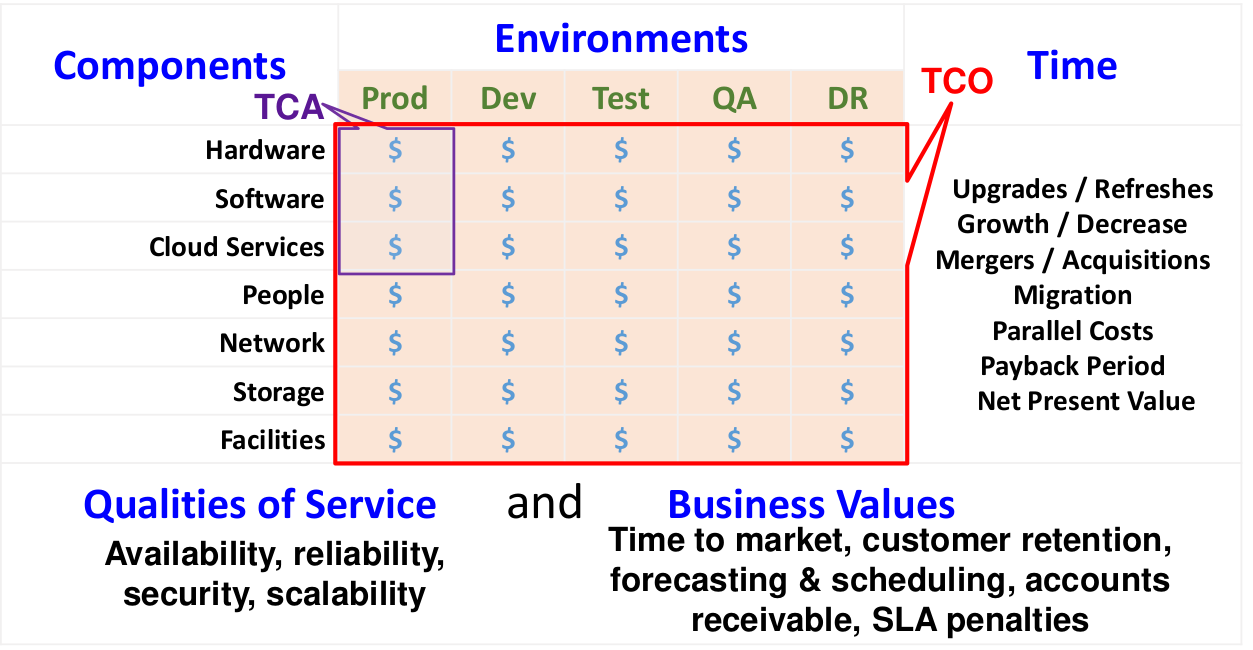
\includegraphics[scale=0.2]{images/TCO-TCA.png}\\
\caption{TCO vs TCA}
\end{figure} 
ogni applicazione ha dei costi legati ad hardware, software, servizi cloud e questi sono i TCA (Total Cost of Acquisition). Vanno anche considerati i costi di gestione del server e dell'applicazione, tipicamente per ogni 30 server occorre un IT admin (anche se non è una sola persona, possono essere anche di più che poi completano un full time equivalent, ovvero 40h/sett).\\ Bisogna anche considerare altre voci di costo, che sono presenti anche per tutti gli altri ambienti e di tutti i requisiti introdotti prima, come anche dei business values e del tempo: una cosa è il costo di acquisto, ma poi nel tempo dovrò fare degli upgrades software, refresh hardware e quindi tipicamente il TCO si fa su una finestra di 5 anni; spesso il refresh cycle viene stabilito nell'azienda: sul totale dei server, se ne cambieranno periodicamente (non per forza tutti insieme) un certo numero. Spendere decine di milioni per mettere su un ambiente Enterprise è abbastanza comune: a seconda della scelta di avere scale up o scale out ci saranno costi diversi, ma tipicamente il costo di scale out è maggiore; inoltre, la parte che ormai ha un costo predominante del TCO è quella del software come anche il costo del disater recovery (che deve mettere insieme i costi di hardware, software etc... che copre non per forza tutti gli stessi servizi dell'ambiente main site).
\subsection{Rack - z15}
In un ambiente Enterprise, rispetto ad un ambiente x86, posso avere un singolo rack (evoluzione dei mainframe), ne esistono due versioni:
\begin{itemize}
\item z15, ultima versione. Possono girarvi n sistemi operativi
\item LinuxONE, mainframe dedicata la mondo Linux
\end{itemize}
\subsubsection{Hardware z15}
L'hardware viene visto come un data-center in una scatola, composto da n server più i sistemi di storage, networking etc..., è stato progettato per virtualizzare e condividere le risorse: sopra il firmware di virtualizzazione gira lo z/VM, che crea VM dal punto di vista hardware (hypervisor di tipo 1).\\ Su ogni z/VM gira un z/OS e possono essere differenti, o anche un altro hypervisor.Ci sono diverse tipologie di processori:
\begin{itemize}
\item di tipo generale (equivalente delle CPU)
\item alcuni dedicati a fare dei compiti specifici (ad esempio per la gestione dell'I/O)
\item processori dedicati all'accoppiamento di due macchine, per farla sembrare una singola
\item zaaP, ottimizzati per eseguire il codice Java (ottimizzare la garbage collection etc...), sono una configurazione particolare di quelli generali
\item spare processor, di scorta. In questo modo se un'altra delle CPU fallisce, questi entrano in gioco
\end{itemize}
\paragraph{LPAR}suddivisione del sistema z in una macchina logica che viene configurata su misura, viene fatta anche dal punto di vista hardware per efficienza. Le LPAR sono isolate dal punto di vista hardware, in modo che in caso di guasti le altre LPAR rimangono su. Siccome il server z è configurato con diversi LPAR, riesce a stare su per decine di anni (senza fare reboot), possono condividere hardware, ma la memoria deve essere isolata.\\
\paragraph{RAIM - memory sparing}si usano memorie RAIM (Redudant Array Indipendent Memory): ci sono più banchi di memoria, in modo che se uno si rompe ce n'è un altro che ha i dati disponibili. Il RAIM prende il 20\% della memoria diposnibile, e versioni non RAIM non sono disponibili su macchine simili.\\ Lo z15 contiene fino a 108 core a 5.2GHz, fino a 40TB di memoria configurabile, offre anche retro compatibilità fino agli anni 60. Si parla di un "data center in a box", i costi saranno molto elevati.
\subsubsection{Confronto x86}
Sicuramente per avere le stesse prestazioni devo avere molteplici server, e abbiamo visto che al crescere dei server crescono anche i problemi in termini di availability, security etc...
\subsection{Gestione dei picchi di carico}
Un altro problema importante da gestire è calibrare un sistema per gestire i picchi di carico: fare over-provisioning è una soluzione tipica, ma c'è un grande spreco di risorse, quindi prezzi più alti così come anche consumi più alti.\\ Uno degli approcci è quello di usare un ambiente cloud, per sfruttarne l'elasticità, tipicamente per una Enterprise si configura un ambiente dedicato in base al tipo di applicazione. L'utilizzazione tipica dei server sta intorno al 20\%, sotto alto utilizzo siamo introno al 30\%, questo in base allo statistical multiplexing model: in base alla media, posso avere picchi differenti in base all'applicazione. Esistono diversi studi dello statistical multiplexing per cui se mettiamo su un servizio su un server, la probabilità che tutti i server abbiano un picco di richieste è molto bassa (utilizzazione pari ad 1), ci sono diversi server di tipo Enterprise in cui la distanza fra picco e media è bassa.\\ Queste macchine inoltre sono state pensate per lavorare ad utilizzazione al 100\%, il sistema operativo è abituato a girare all' 80-90\% e tutto ciò porta ad avere un utilizzo delle risorse molto ottimizzato.
\subsection{Esempio: pricing di database commerciali}
Di seguito vengono riportati i pricing per l'utilizzo dei database di alcune Enterprise:
\subsubsection{IBM D2}
I prezzi per il servizio D2 di IBM non sono pubblici, ma vanno richiesti contattando l'azienda.\\\\
\begin{table}
\begin{tabular}{ | c c c c | }
\hline
 & Community edition & Standard edition & Advanced edition\\
\hline 
Price(perpetual) & Free/unsupported & Contact us & Contact us\\
\hline
Price(subscription) & N/A & Contact us & Contact us\\
\hline
Caps & 4 cores & 16 cores & Unrestricted\\
 & 16 GB RAM & 128 GB RAM &  \\
\hline
Free trial period & Free & Development or & Development or\\
 & indefinetly & production & production\\
\hline
License & Development or & Development or & Development or\\
 & production & production & production\\
\hline
Metric & Not applicabile & Virtual process & Virtual process\\
 & & core & core\\
\hline
Features & All features & All features & All features\\
\hline
\end{tabular}
\caption{IBM D2 pricing}
\end{table}
\FloatBarrier
notiamo come nella metrica, oltre 
\subsubsection{Oracle DB}
\subsubsection{Microsoft SQL}
\begin{table}[ht]
\begin{tabular}{ c c c c }
\hline
Edizioni & Prezzo Open & Modello & Disponibilità per\\
 & No Level & di licenza & il canale\\
\hline
Enterprise & \$13,748 & Pacchetto da & Contratti multilicenza,\\
 & & 2 core & hosting\\
\hline
Standard - per core & \$3,586 & Pacchetto & Contratti multilicenza,\\
 & & da 2 core & hosting\\
\hline
Standard - server & \$899 & Server & Contratti multilicenza,\\
 & & & hosting\\
\hline
Standard - CAL & \$209 & CAL & Contratti multilicenza,\\
 & & & hosting\\
\hline
Developer & Gratuito & Per utente & Download\\
 & & & gratuito\\
\hline
Web & Rivolgersi ai & Non applicabile & Solo hosting\\
 & partner di hosting & &\\
 & per informazioni & &\\
 & sui prezzi & &\\
\hline
Express & Gratuito & Non applicabile & Download\\
 & & & gratuito\\
\hline
\end{tabular}
\caption{Microsoft SQL pricing (2019}
\end{table}
\FloatBarrier
Nel caso di Microsoft SQL, dove i prezzi sono espressi in dollari, la metrica fa riferimento ai singoli core di CPU. Inoltre, vengono forniti maggiori dettagli sul \textcolor{blue}{\href{https://www.microsoft.com/it-it/sql-server/sql-server-2019-pricing}{sito}}.
\subsubsection{DynamoDB}
\end{document}